\documentclass[conference]{IEEEtran}
\usepackage{tikz}
\usepackage{graphicx}
\usepackage{float}

\usetikzlibrary
	{ arrows
	, positioning
	, fit
	, shapes
	, calc
	}

\begin{document}

\title{The Hadoop Framework}

\author{\IEEEauthorblockN{Stephen O'Brien}
\IEEEauthorblockN{R00048347}
\IEEEauthorblockA{Cork Institute of Technology}
\today
}

\maketitle
\suppressfloats

\begin{abstract}
This report details an overview of Hadoop, its components and architecture including how Hadoop achieves it's level of fault tolerance and scalability.
\end{abstract}

% creates the second title. It will be ignored for other modes.
\IEEEpeerreviewmaketitle



\section{Introduction}
Hadoop is a framework for data processing at a large scale, born from the cross over of the \emph{Nutch} web crawler and two papers 
released by Google - \emph{MapReduce: Simplified Data Processing on Large Clusters} \cite{mapreduce} and \emph{The Google File System} \cite{gfs}. 
The Google File System (GFS) paper outlines the architecture for Googles proprietary distributed filesystem, used for large distributed applications, while the MapReduce paper outlines a programming model for processing large datasets. Apache Nutch \cite{nutch}, an early large scale web crawler, was created in the early 2000's by Doug Cutting and Mike Cafarella, after the release of the GFS paper they decided to look into building an open source implementation of GFS, they called it NDFS, the Nutch Distributed File System. Not long after the release of the MapReduce paper, the Nutch developers also had a working implementation of MapReduce within Nutch. It was from this code base that the initial version of Hadoop was formed \cite{nutch2hadoop}.

\section{Hadoop Architecture}
At a high level Hadoop consists of two layers, a compute layer, \emph{YARN} (Yet Another Resource Negotiator) and a storage layer, \emph{HDFS} (Hadoop Distributed File System). \emph{YARN} provides API's to request work to be scheduled on the cluster. These API's are generally consumed by frameworks such as \emph{Apache Spark} or \emph{MapReduce}, these frameworks then expose higher level API's allowing users to write applications and not have to worry about interacting directly with \emph{YARN}.

The storage layer, \emph{HDFS}, was built for very large files, 100GB's/TB's or larger and was built to run on commodity hardware. It manages large files by splitting them up into a sequence of blocks and storing the blocks across machines in a cluster of storage nodes \cite{hdfs}.

Above the compute and storage layers sits the frameworks which use \emph{YARN}'s API's to schedule work across the cluster. \emph{MapReduce} is one of these frameworks, but there are many more - Apache Spark, Hive, Pig, to name a few. See Figure ~\ref{highlevelarch} for a simple visual overview.

\begin{figure}[ht]
\centering
\scalebox{0.5}{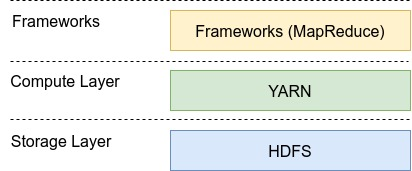
\includegraphics[width=\textwidth]{images/HadoopHighLevelArch.jpeg}}
\caption{High Level Overview of Hadoop Architecture}
\label{highlevelarch}
\end{figure}

\subsection{HDFS}
\emph{HDFS} is a distributed file system, designed to handle large datasets. \emph{HDFS} embraces the idea that a write-once read-many data processing pattern is the most efficient. Typically within Hadoop an analysis of a dataset would use the whole of, or most of, the dataset so for \emph{HDFS} the read time of the entire dataset is more important than the latency of reading the first item in the dataset \cite{hdfs}. 

The architecture of HDFS comprises of a single \emph{NameNode} and multiple \emph{DataNodes}, NameNodes can also be federated, whereby multiple NameNodes work independently but use the same underlying DataNodes. The NameNode manages the filesystem namespace, it uses \emph{inodes} to represent files, directories and related metadata. File contents are split into blocks, which are replicated and stored across multiple DataNodes. The NameNode also manages this mapping of file contents to blocks across DataNodes. A read of file data from a HDFS client will first request block locations of the file from the NameNode, once the locations are received the client uses these locations to read blocks from the nearest DataNode \cite{hdfs}. This read operation is outlined in Figure \ref{clientread}.

\begin{enumerate}
\item Client requests block location information from the NameNode.
\item The NameNode responds giving the closest DataNode to the client for each block requested.
	\item \begin{enumerate}
     \item One of the block locations was local, the client requests this directly.
     \item Another block was stored on a DataNode on another rack, the client also requests this directly.
   \end{enumerate}
\end{enumerate}


\begin{figure}[ht]
\centering
\scalebox{0.5}{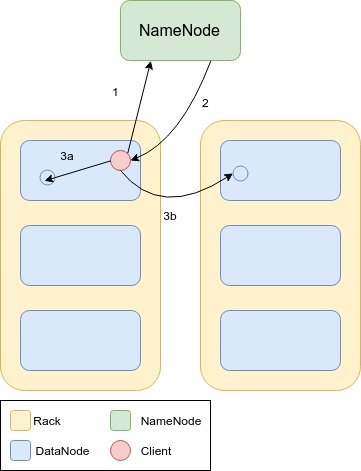
\includegraphics[width=\textwidth]{images/clientread.jpg}}
\caption{High Level Overview of HDFS Architecture}
\label{clientread}
\end{figure}

Loss of a NameNode means complete loss of all files that NameNode was managing as it is the single source which knows how to reconstruct files from their constituent blocks. One way to prevent this is to run a \emph{secondary NameNode} \cite{secnamenode} which takes snapshots of the primary NameNode's state over time, if the primary NameNode fails the secondary can take over.

\subsection{YARN}
YARN is Hadoop's cluster resource management system. It provides an API for working with cluster resources, this allows management of resources to be abstracted away from developers when using frameworks such as MapReduce - MapReduce exposes a higher level API using YARN underneath to manage resources. YARN consists of two daemons - a per-cluster \emph{ResourceManager} and a set of \emph{NodeManagers} \cite{yarn}.

A NodeManager runs on every node in the cluster, they are responsible for monitoring resource availability, tracking and alerting on faults, and managing the lifecycle of \emph{containers}. Containers execute application specific processes within bounded resources, YARN can run containers and limit resources as processes directly or by using Linux \emph{cgroups} \cite{yarncgroups}.

\begin{figure}[ht]
\centering
\scalebox{0.5}{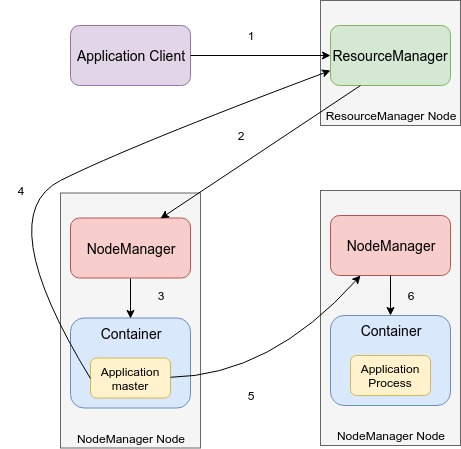
\includegraphics[width=\textwidth]{images/yarn.jpg}}
\caption{YARN application initialization overview}
\label{yarn}
\end{figure}

Figure \ref{yarn} outlines the initialization of an application.

\begin{enumerate}
\item Application client submits a request to launch an \emph{Application Master}. The Application Master is the co-ordinator for the submitted application. For example, with MapReduce the application master handles requesting resources from the ResourceManager which will schedule containers for MapReduce tasks, these containers will be managed by the NodeManagers. For each MapReduce job there would be one Application Master.
\item The ResourceManager searches for a NodeManager which has the resources capable of launching the Application Master container.
\item The chosen NodeManager launches the Application Master container.
\item The Application Master requests more resources from the ResourceManager.
\item Once the resources have been allocated, the Application Master talks to the NodeManager directly to launch the container for the application process. In the case of MapReduce, this application process would be a map or reduce task.
\end{enumerate}

\subsection{MapReduce}
The MapReduce paper \cite{mapreduce} introduced a programming model for data generation and data processing. The model defines a computation which takes a set of key/value pairs as input and produces a set of key/value pairs as output.
This computation is composed of two different functions, \emph{Map} and \emph{Reduce}. \emph{Map} takes a key value pair as input and produces a set of \emph{intermediate} key/value pairs. These intermediate key/value pairs are processed by the \emph{MapReduce} library, which groups all values associated with each key and sends them to the \emph{Reduce} function. \emph{Reduce} takes the key and its set of values and produces zero or more outputs, depending on what the writer of the \emph{Reduce} function wanted to learn from the data.

\emph{MapReduce} is a framework in Hadoop implementing the above programming model. Within this framework the unit of work is called a \emph{job}, it abstracts job resource management from writers of \emph{MapReduce} applications, calling the YARN API internally to have it schedule and manage jobs. Hadoop executes a job by splitting it into \emph{tasks} of which there are two kinds - map tasks and reduce tasks. The input of a job is divided into splits \cite{mapreduce}, there is one map task per split. This makes it highly parallelizable, more splits equals less processing time. However, if splits are too small the overhead of managing them will dominate job execution time.

Split sizes are generally the same size as the block size in HDFS (whose default is 128MB) \cite{hdfs}. The advantage being the block size is the largest slice of input guaranteed to be on a node. If the split size spanned two or more blocks it would be highly unlikely any single node had all those blocks.

Hadoop tries to run map tasks on a node where the input to the task resides, this helps to reduce cluster bandwidth usage as data does not have to be transferred between nodes to feed map tasks - the higher the data locality the less data has to be copied from node to node. Sometimes this is not possible, so the job scheduler will try to use a node on the same rack (a rack is the physical machine nodes are located on) - failing that it will try off rack nodes. The point of this process is to try to keep data locality as high as possible when executing map tasks.

Once a map task is complete, it writes the output to the local filesystem and not to HDFS, the map outputs are intermediate and will be discarded once the reduce task consumes them. For reduce, there is generally no data locality , the input is usually the output of all map tasks (there can be partitioning of reduce tasks also).

\section{Fault Tolerance}
Block replication in HDFS allows for a high level of fault tolerance. When data is stored it is replicated across multiple DataNodes. If any of these nodes is lost there will be at least $n - 1$ DataNodes left which contain the blocks the failed node had - where $n$ is the replication level configured in HDFS \cite{hdfs}.

Within YARN, when a NodeManager fails, the ResourceManager detects this as the failed Nodemanager will no longer be sending a heartbeat. The ResourceManager will then mark all containers on the failed node as \emph{killed}, finally reporting all failures to Application Masters. It is the responsibility of the Application Masters to handle node failure events and re-schedule work if necessary \cite{yarn}.

If an Application Master fails, the ResourceManager may restart it, however there is no support for restoring state to Application Masters. Re-synchronization of any processes the Application Master was managing is also not the responsibility of Hadoop, it is left up to each individual Application Master \cite{yarn}.

Container failure is also left to the Application Masters, or the frameworks running on top of Hadoop. The ResourceManager will collect and propagate container exit events to Application Masters, leaving them handle the semantics for possible recovery. In MapReduce, for example, if an Application Master receives a container failure event it will try to reschedule the map or reduce tasks that failed \cite{yarn}.

In Hadoop 2.0 HDFS HA was introduced \cite{hadoopha}. This allows a pair of NameNodes to be clustered in an active/passive configuration. If the active node fails the passive node takes over. This is achieved by a component called the \emph{failover controller}. Each NameNode runs a failover controller process which monitors the NameNode and triggers a failover if the NameNode fails. There are two types of failover: \emph{graceful failover} which could be initiated by manually taking the node down, and \emph{ungraceful failover} in which it is not possible to be sure the node has actually stopped running (e.g. network partition). In the latter case the HA implementation tries to make sure the previous active NameNode does not cause any damage.

\section{Scalability And Throughput In Applications}
HDFS is designed to split data into multiple blocks and store them across a cluster of DataNodes. By doing this, applications that run on top of Hadoop can achieve high levels of parallelism when processing the data. For example with MapReduce a task is created to process each block of data simultaneously. Second to this NodeManagers in YARN will try their best to allocate MapReduce tasks to nodes where the data resides increasing data-locality. In doing this, they reduce the amount of cluster bandwidth in use and also the amount of time it takes the task to read the data it needs, thereby increasing the throughput of the task and cluster overall. This one of the main ways in which Hadoop achieves high levels of throughput.

To improve on this, NameNodes (NN) in HDFS are \emph{Rack Aware} \cite{rackaware}. This means that NN's know which DataNodes are located in which physical racks. If an NN cannot co-locate a task with the data it needs to consume it can try to allocate a task on a rack where at least one DataNode has the data which the task needs to work on. This too helps to decrease cluster bandwidth usage, and increase the throughput of the executing task.

\section{Hadoop vs. Spark}
Hadoop was developed with batch processing in mind - non-interactive processing of data which has already been stored, and it's storage is tied specifically to HDFS. Because of this architecture certain types of data processing do not fit well. A good example is machine learning algorithms which use gradient descent. These apply a function to the same dataset, optimizing parameters trying to find a global minimum for the cost of the function. Each iteration maps to a MapReduce job, but each iteration will also need to reload its data from disk, which incurs a large performance penalty. 

Spark on the other hand was designed with these types of jobs in mind. Its data model is based around the concept of \emph{resilient distributed datasets} (RDD) which are read-only collections of objects partitioned across a cluster of machines \cite{spark} . Processing of these datasets is done in memory which is much more suited to the types of jobs Hadoop would have performance penalties for, as mentioned above. Spark can read datasets, constructing RDD's, from files in filesystems such as HDFS or S3 - it is not tied to HDFS alone. 

Spark also has fault tolerance guarantees similar to Hadoop. RDD's achieve fault tolerance through the concept of \emph{lineage}. When a partition of an RDD is lost, the RDD will have enough information to be able to rebuild just that lost partition.

Spark is also decoupled from it's underlying cluster implementation. The original version ran on \emph{Mesos} \cite{mesos} but as Spark has matured it has gained support for a number of other cluster management systems such as Kubernetes and even YARN.

\begin{thebibliography}{1}

\bibitem{nutch}
http://nutch.apache.org/.

\bibitem{nutch2hadoop}
https://issues.apache.org/jira/browse/NUTCH-193.

\bibitem{mapreduce}
Jeffrey Dean and Sanjay Ghemawat, \emph{MapReduce: Simplified Data Processing on Large Clusters}, December 2004.

\bibitem{gfs}
Sanjay Ghemawat, Howard Gobioff, and Shun-Tak Leung, \emph{The Google File System}, October 2003.

\bibitem{hdfs}
Konstantin Shvachko, Hairong Kuang, Sanjay Radia, Robert Chansler, \emph{The Hadoop Distributed File System},  May 2010.

\bibitem{secnamenode}
https://hadoop.apache.org/docs/stable/hadoop-project-dist/hadoop-hdfs/HdfsUserGuide.html.

\bibitem{yarn}
Vavilapalli et al., \emph{Apache Hadoop YARN: Yet Another Resource Negotiator}, October 2013.

\bibitem{yarncgroups}
https://hadoop.apache.org/docs/stable/hadoop-yarn/hadoop-yarn-site/NodeManagerCgroups.html.

\bibitem{rackaware}
https://hadoop.apache.org/docs/stable/hadoop-project-dist/hadoop-common/RackAwareness.html.

\bibitem{spark}
Matei Zaharia, Mosharaf Chowdhury, Michael J. Franklin, Scott Shenker, Ion Stoica, \emph{Spark: Cluster Computing with Working Sets}.

\bibitem{mesos}
http://mesos.apache.org/.

\bibitem{hadoopha}
https://hadoop.apache.org/docs/stable/hadoop-project-dist/hadoop-hdfs/HDFSHighAvailabilityWithNFS.html

\end{thebibliography}
\end{document}


